\graphicspath{{chapters/04/}}

\chapter{Tumor Evolution Studies via NGS data}
Tumor board: organism research oriented (and not) hospitals, patient not strictly assigned to one doctor but many specialist. E.g. oncologists, pathologists, geneticists...
\\
TUmor boards teach young doctors how to manege difficult events.
\section{Tumor evolution}
%reference paper Tumour heterogeneity and resistance to cancer therapies
What are the somatic events that occur during tumor genesis/evolution and when do they arise?\\
First of all, remember that every cancer cell was once a healthy celss that underwent some stress (UV light, radiation...).\\
Typical traits of cancer are:
\begin{itemize}
\item Cancer is a dynamic disease, that's why evolution of the desease is so important to track.
\item During the course of disease, cancers generally become more
heterogeneous, which is often related to treatment resistance.
\item The bulk tumor includes a diverse collection of cells harboring distinct molecular signatures with differential levels of sensitivity to treatment.
\item This heterogeneity might result in a non-uniform distribution of genetically
\item distinct tumour-cell subpopulations across and within disease sites (spatial heterogeneity) or temporal variations in the molecular makeup of cancer cells (temporal heterogeneity)
\end{itemize}

Heterogeneity is a big obstacle in cancer treatment. Two characteristics to keep in mind are:
\begin{itemize}
\item Heterogeneity provides the fuel for resistance; therefore, an accurate assessment of tumor heterogeneity is essential for the development of effective therapies.
\item Multiregion sequencing, single-cell sequencing, analysis of autopsy samples, and longitudinal analysis of liquid biopsy samples are all emerging technologies with considerable potential to dissect the complex clonal architecture of cancers. 
\end{itemize}

However, techniques to study tumor heterogeneity are hindered by intra-patient heterogeneity: spatial and temporal. 


\begin{figure}[htbp!]
	\centering
	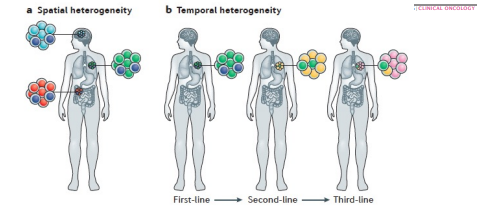
\includegraphics[width=0.7\textwidth]{heterogeneity.png}
	\caption{\label{fig:hetero} a) Spatial heterogeneity denoes an uneven distribution of cancer subclones across different regions of the primary tumor and/or metastatic sites. b) Temporal heterogeneity refers to variations in the molecular makeup of a single lesion over time, either as a result of natural progression of the tumor or as a result of exposure to selective pressures created by clinical interventions. Colours denote the presence of subclones with different genetic features.}
\end{figure}

Let's focus for the moment only on spatial, and not temporal, tumor heterogeneity. \\
Certain cells respond to treatment and some don't. Red = cell resistant to drug, blue = cell sensitive to drug. 

\begin{figure}[htbp!]
	\centering
	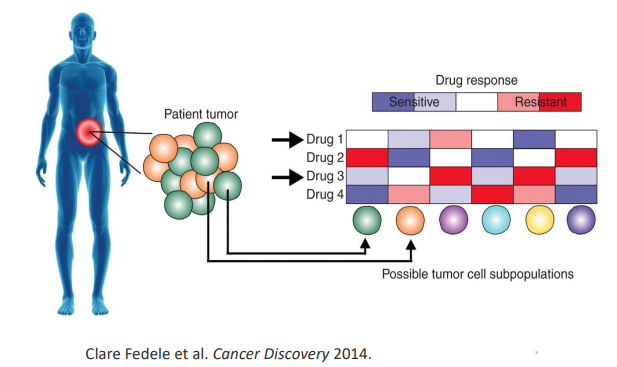
\includegraphics[width=0.7\textwidth]{treatment.png}
	\caption{\label{fig:treatment} Schematic view of what a heterogeneous cancer may look like.}
\end{figure}

Linear evolution vs branching evolution.\\
The feature of this set of cells over time and for some reason either the new population replaces the older, or there's a branching and the tumor mass becomes heterogeneous.\\
\begin{figure}[htbp!]
	\centering
	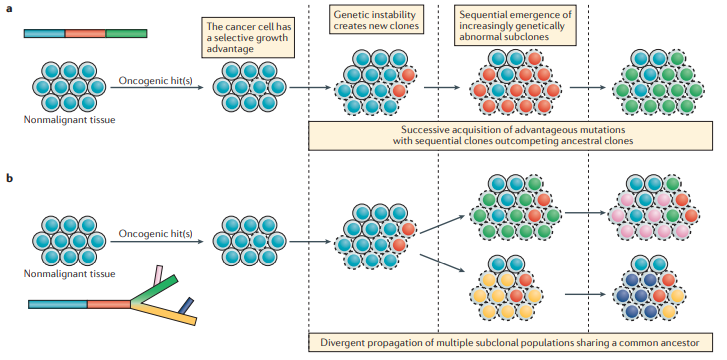
\includegraphics[width=0.7\textwidth]{branching.png}
	\caption{\label{fig:branching} Schematic view of what a heterogeneous cancer may look like.}
\end{figure}

a) everything branches out from the monoclonal origin, but b) polyclonal origin, indipendent metastatic processes. Cells from indipendent lesions meet and form a highly diverse metastatic tumor.\\

A major concept: is treatment resistance encoded in the original sets or is driven by the treatment itself?\\
Selection of clones tat provide resistance, or transofmration of clones under teatment pressure. 

\begin{figure}[htbp!]
	\centering
	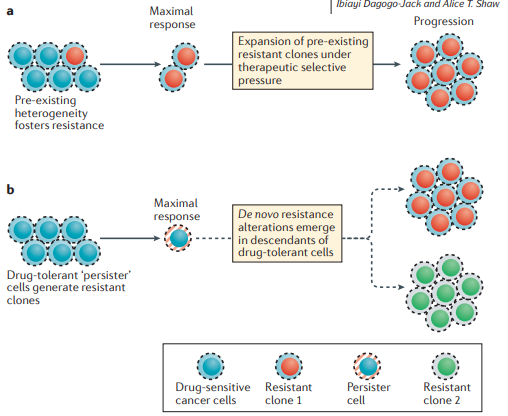
\includegraphics[width=0.7\textwidth]{response.png}
	\caption{\label{fig:response} Schematic view of what a heterogeneous cancer may look like.}
\end{figure}

\section{From sketches to sequencing data evolution information}
Multiple individuals and on the left side there's evollution inferred frolm the data. On the right, assessment that suggests that it's compatible with monoclonal seeding. \\
What lesions ocured first and which is the model that fits better the data.\\

\subsection{Tumor evolution and heterogeneity}
To summarize, there are the difficult tasks one has to deal with when studying tumor data:
\begin{itemize}
\item intra tumor heterogeneity;
\item inter tumor/intra patient heterogeneity;
\item Inter-patient heterogeneity;
\item clinical/treatment relevance;
\item time dependency;
\item admixture DNA (tumor purity);
\end{itemize}

However, if recognized, they can also provide for insightful hints int he analysis.\\

\subsubsection{Admixture}
Tissue from any source we have multiple cell types, each present with a given ratio.\\
Deconvultion looking at NGS data. Lesion 100\% pure if the contamination of the adm of tumor cells is very low. \\
This info (purity = 1- adm) is improtant for 
\begin{itemize}
\item agressvness
\item every interpetation of somatic data needs to be interpreted in the contex of tumor purity. Lesion is clonal if all tumor cells have it, a less present lesion instead might be subclonal.
\end{itemize}

\subsection{Useful feature from NGS data}
\begin{itemize}
\item Polymorphic information that is presentin the genetics of every individual. SNPs are very helpful in all somatic analysis.
\item MAF= minor allele frequency, freq a ehich the allele at a polymorphic site is present in a population. Used for SNPs in general.
\item AF= allelic fraction, how many times ina specific locus a base is represented. How mnay reads represent the alternative allele, how muh support. 
\end{itemize}

\subsection{Allelic Fraction (AF) properties}
Most important algorithms: how to exploit informative SNPs for interpetation tumor studies.\\

\begin{itemize}
\item Informative SNPs are sites in which the individual has a heterozygous base. For each SNPs we can calculate the AF.
\item Neutral Reads
\item Beta measure that No lesion and the two allelic equally represented then beta is one. With beta moving towards zero we have a measure 
\item Nref
\end{itemize}

AF: an info SNPs with loss of heterogeneity due to monoallelic los sis either 0 or 1, anything in the middle is an indication of either admixture or subclonality of the lesion.

\begin{figure}[htbp!]
	\centering
	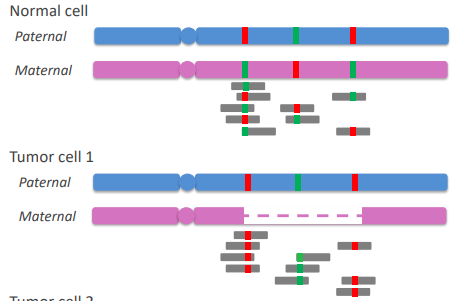
\includegraphics[width=0.7\textwidth]{af_properties.png}
	\caption{\label{fig:af_properties} Schematic view of what a heterogeneous cancer may look like.}
\end{figure}

An example of the use of AF and beta measures for tumor data analysis in depicted in 

\begin{figure}[htbp!]
	\centering
	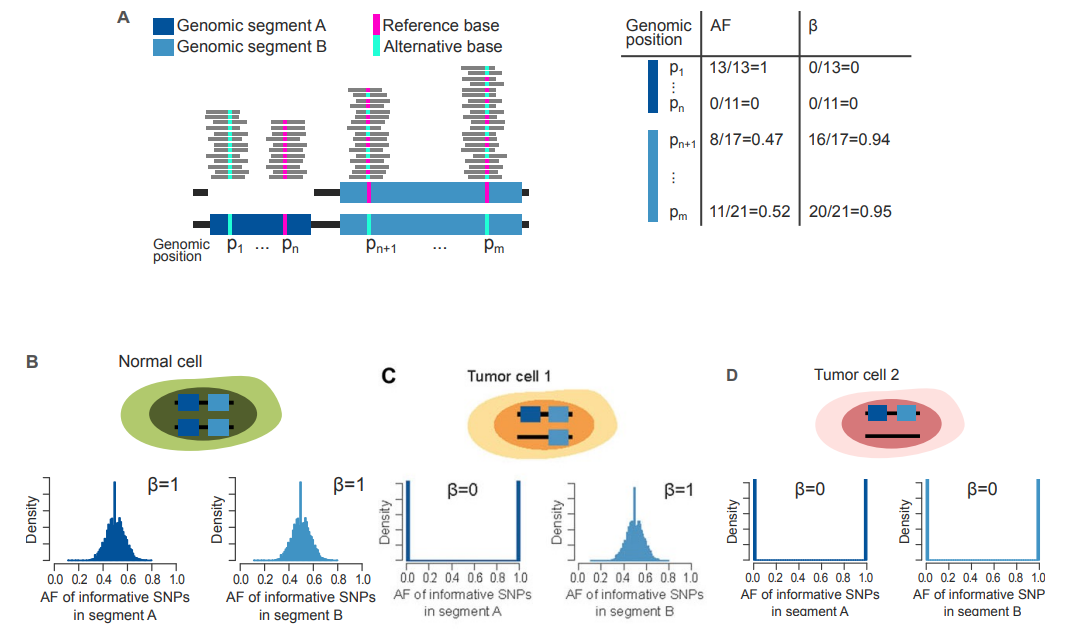
\includegraphics[width=0.8\textwidth]{a.png}
	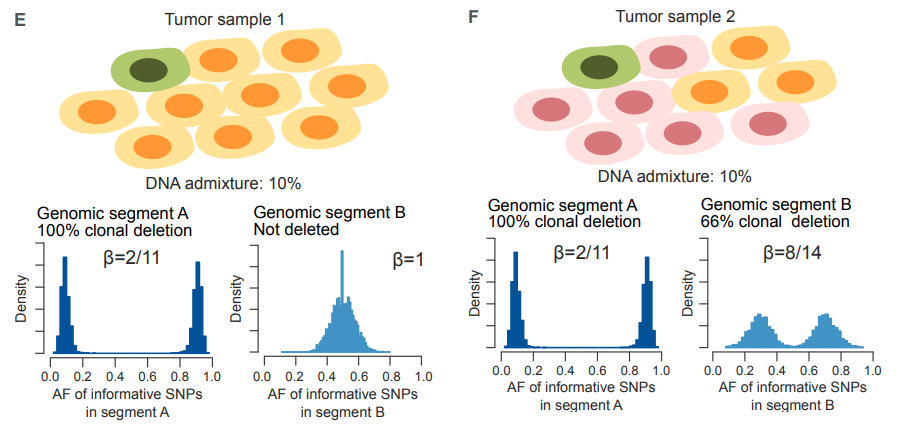
\includegraphics[width=0.8\textwidth]{b.png}
	\caption{\label{fig:a_b} 
	\textbf{A)}Example of the allelic fraction (AF) and beta ($\beta$) in computed in five genomic positions ($p_1$ to $p_m$). Positions $p_1$ to $p_n$ are within a hemizygous deleted genomic segment A, while genomic positions $p_{n+1}$ to pm lie within a wild type genomic segment B.\\
\textbf{(B-D)} Examples of a normal cell and two different tumor cells. Tumor cells 1 and 2 differ for the status of genomic segment B. Histograms below cell cartoons report the expected distribution of the allelic fraction of SNPs in genomic segments A and B together with the associated beta values.\\
\textbf{(E-F)} Examples of two different tumor samples. Tumor sample 1 includes one normal cell and nine tumor cells with deleted genomic segment A and wild type genomic segment B. Tumor sample 2 differs from tumor sample 1 in the presence of six tumor cells with a hemizygous deletion of genomic segment B.
Expected distribution of the AF of informative SNPs together with estimated beta are depicted below each tumor sample cartoon.}
\end{figure}

In each genomic segments there are many info SNPs, but if there is not any, there's nothing we can say.

\section{Coverage and AF properties}
Does the mean coverage of the experiment impact on the ability to use the AF properties?\\
Intuitively, the deeper the sequencing the more likely it is to distinguish distribution that are not so close to each other. It is especially important when $\beta$ is close to zero. An example is shown in figure \ref{fig:beta}.

ccc

\section{Computing Beta}
A Beta for each genomic segment S:
\begin{itemize}
\item compute the observed distribution of the AF of
informative SNPs in S
\item find the values of Beta and Nref such that the expected
distribution of the AF matches the observed AF
\item compute uncertainty around Beta as a function of:
	\begin{itemize}
	\item the mean coverage of S
	\item the number of informative SNPs in S
	\end{itemize}
\end{itemize}

\section{Global vs Local Estimates of admixture}
We'll discuss two types of sample and how to determine cell population (admixture).

In sample one depicted in figure \ref{fig:sample1} there's a clonal cell population, meaning no heterogeneity. On the x axis we have genomic coordinates indexed by informative SNPs for that individual.
\\
For all the info SNPs present in this chunk of DNA, we see drops in AF that are smaller or wider, but more or less for each one of those lesions (drops), representing a drop or a gain in the amount of DNA is almost identical in all of these chunks.  
The representation of the lesions is supported by the same data along the stretch of DNA.
Thinking in terms of how much the AF distribution from 0 and 1 and the center is basically the same across all of them. Meaning, the level of admixture, both globally and locally, is the same. \\
The amount of cells that have the first, second, third lesion etc. is the same.

\begin{figure}[htbp!]
	\centering
	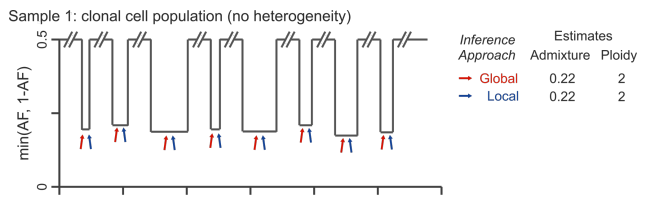
\includegraphics[width=0.7\textwidth]{sample1.png}
	\caption{\label{fig:sample1}}
\end{figure}

In the picture \ref{fig:sample2} below we can see another sample.
We can clearly discover multiclonal cell population. The depth of the lesion is proportional to the number of cells that carry the lesion.
In this case the definitions of local and global admixture change: a \textbf{global} value is a global value of tumor purity, a local value is a value of the clonality of the lesion in the diseased cell population.

\begin{figure}[htbp!]
	\centering
	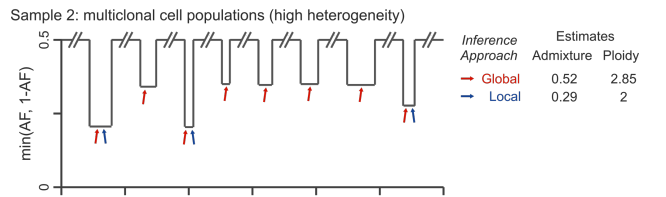
\includegraphics[width=0.7\textwidth]{sample2.png}
	\caption{\label{fig:sample2} }
\end{figure}

\subsubsection{Estimate of DNA admixture (1-Purity)}
We will now translate the concepts expressed in the previous sections in a 2-dimensional space, as shown in figure \ref{eq:adm}.

\begin{wrapfigure}{l}{0.5\textwidth}
	%\centering
	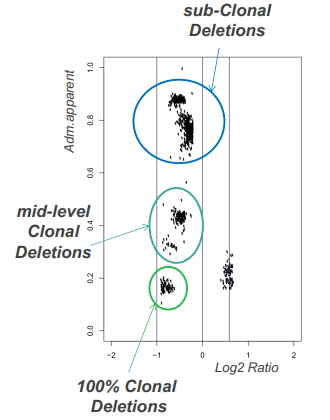
\includegraphics[width=0.7\linewidth]{adm.png}
	\caption{\label{fig:adm} Every dot is one genomic segment, they form clusters.  }
\end{wrapfigure}

On the x axis we have the Log2 ration measure and on the y axis the admixture apparent, which is proportional to the beta  value.\\
The Log2 Ratio is basically tumor over normal in the log2 space. It allows to interpret info about every segment int he genome when coupled with the beta measure.
\\
The admixture apparent is calculated as 

\begin{equation} \label{eq:adm}
\textit{Adm. apparent} = \frac{\beta}{2-\beta}
\end{equation}

This measure associates an apparent DNA admxiture to each monoallelic deletion. It is useful to calculate the clonality values, for which the formula is: 

\begin{equation}
\textit{Clonality:} \frac{1 - \textit{Adm. apparent}}{1 - \textit{Adm. global}}
\end{equation}

The lowest cluster is the one used to assess admixture and the other ones are subclonal lesions.\\
Moreover, the closest the points are, the most probable it is that the lesions happened close in time, and viceversa.

\section{A challenging case (PR-2741}
Data of a real case of prostate cancer in which we can see a clear drop in coverage in region 2 of the 5th chromosome. The DNA present in region 2 could come either from admixting cells or from cells that do not have the deletion. \\
Looking at the AF of region 1, 2, 3 both from the tumor and the match normal normal sample we observe more or less the same two modes of distribution.\\
In the tumor sample in fact we do not see two peaks in 0 and 1 as expected. It could be signal of intervening normal cells, that bring the modes to the center, or subclonality event. \\


























